\documentclass[12pt,a4paper]{article}

%% ── Encoding & Fonts ─────────────────────────────────────────────────────────
\usepackage[T1]{fontenc}
\usepackage[utf8]{inputenc}


%% ── Page Layout ──────────────────────────────────────────────────────────────
\usepackage[
  top=2.5cm,
  bottom=2.5cm,
  left=2.8cm,
  right=2.8cm,
  headheight=25pt
]{geometry}
\usepackage{setspace}
\onehalfspacing

%% ── Mathematics ──────────────────────────────────────────────────────────────
\usepackage{amsmath,amssymb,amsthm,mathtools}

%% ── Tables ───────────────────────────────────────────────────────────────────
\usepackage{booktabs}
\usepackage{array}
\usepackage{multirow}
\usepackage{longtable}
\usepackage{tabularx}

%% ── Graphics & Colour ────────────────────────────────────────────────────────
\usepackage{graphicx}
\usepackage[dvipsnames,table]{xcolor}
\usepackage{tikz}
\usetikzlibrary{arrows.meta,positioning,shapes.geometric,calc,fit,backgrounds,decorations.pathreplacing}
\usepackage{pgfplots}
\pgfplotsset{compat=1.18}

%% ── Boxes ────────────────────────────────────────────────────────────────────
\usepackage[most]{tcolorbox}
\tcbuselibrary{breakable,skins,theorems}

%% ── Section Formatting ───────────────────────────────────────────────────────
\usepackage{titlesec}
\titleformat{\section}{\large\bfseries\color{keyblue}}{\thesection.}{0.6em}{}[\vspace{-2pt}{\color{keyblue}\rule{\linewidth}{1pt}}]
\titleformat{\subsection}{\normalsize\bfseries\color{keyblue!80!black}}{\thesubsection}{0.6em}{}
\titleformat{\subsubsection}{\normalsize\itshape\color{keyblue!60!black}}{\thesubsubsection}{0.6em}{}

%% ── Captions ─────────────────────────────────────────────────────────────────
\usepackage{caption}
\captionsetup{font=small,labelfont=bf,margin=1cm}

%% ── Lists ────────────────────────────────────────────────────────────────────
\usepackage{enumitem}
\setlist[itemize]{noitemsep,topsep=4pt,label={\color{keyblue}\textbullet}}
\setlist[enumerate]{noitemsep,topsep=4pt}

%% ── Headers & Footers ────────────────────────────────────────────────────────
\usepackage{fancyhdr}
\pagestyle{fancy}
\fancyhf{}
\fancyhead[L]{\small\textit{\color{keyblue!80!black}Gradient Dynamics and Optimization in Deep Networks}}
\fancyhead[R]{\small\textit{\color{keyblue!80!black}Unified Technical Note}}
\fancyfoot[C]{\small\thepage}
\fancyfoot[L]{\small\color{gray!60}v2.0 — Extended Edition}
\renewcommand{\headrulewidth}{0.6pt}
\renewcommand{\headrule}{\hbox to\headwidth{\color{keyblue}\leaders\hrule height \headrulewidth\hfill}}

%% ── Hyperlinks ───────────────────────────────────────────────────────────────
\usepackage[
  colorlinks=true,
  linkcolor=MidnightBlue,
  citecolor=MidnightBlue,
  urlcolor=MidnightBlue,
  bookmarks=true,
  pdftitle={Gradient Dynamics and Optimization in Deep Networks}
]{hyperref}

%% ── Custom Colours ───────────────────────────────────────────────────────────
\definecolor{keyblue}{RGB}{0,63,114}
\definecolor{lightgray}{RGB}{245,245,245}
\definecolor{accentgold}{RGB}{180,140,0}
\definecolor{darkred}{RGB}{150,30,30}
\definecolor{emerald}{RGB}{0,110,80}
\definecolor{plum}{RGB}{100,30,100}
\definecolor{titlegray}{RGB}{40,40,40}
\definecolor{subtlegray}{RGB}{250,250,252}

%% ── Custom Box Environments ──────────────────────────────────────────────────
\newtcolorbox{keybox}[1][Key Result]{
  enhanced, breakable,
  colback=keyblue!5!white,
  colframe=keyblue,
  fonttitle=\bfseries\small\color{white},
  coltitle=white,
  attach boxed title to top left={yshift=-2mm, xshift=4mm},
  boxed title style={colback=keyblue, colframe=keyblue, arc=2pt},
  title=#1,
  left=8pt, right=8pt, top=10pt, bottom=6pt, arc=4pt,
  drop shadow={opacity=0.08}
}

\newtcolorbox{critbox}[1][Critical Assessment]{
  enhanced, breakable,
  colback=darkred!4!white,
  colframe=darkred!70!black,
  fonttitle=\bfseries\small,
  attach boxed title to top left={yshift=-2mm, xshift=4mm},
  boxed title style={colback=darkred!80!black, colframe=darkred!80!black, arc=2pt},
  coltitle=white,
  title=#1,
  left=8pt, right=8pt, top=10pt, bottom=6pt, arc=4pt
}

\newtcolorbox{extbox}[1][Extension]{
  enhanced, breakable,
  colback=accentgold!6!white,
  colframe=accentgold,
  fonttitle=\bfseries\small,
  attach boxed title to top left={yshift=-2mm, xshift=4mm},
  boxed title style={colback=accentgold!90!black, colframe=accentgold, arc=2pt},
  coltitle=white,
  title=#1,
  left=8pt, right=8pt, top=10pt, bottom=6pt, arc=4pt
}

\newtcolorbox{practbox}[1][Engineering Practice]{
  enhanced, breakable,
  colback=emerald!4!white,
  colframe=emerald!80!black,
  fonttitle=\bfseries\small,
  attach boxed title to top left={yshift=-2mm, xshift=4mm},
  boxed title style={colback=emerald!80!black, colframe=emerald!80!black, arc=2pt},
  coltitle=white,
  title=#1,
  left=8pt, right=8pt, top=10pt, bottom=6pt, arc=4pt
}

\newtcolorbox{gapbox}[1][Gap / Correction]{
  enhanced, breakable,
  colback=plum!4!white,
  colframe=plum!70!black,
  fonttitle=\bfseries\small,
  attach boxed title to top left={yshift=-2mm, xshift=4mm},
  boxed title style={colback=plum!70!black, colframe=plum, arc=2pt},
  coltitle=white,
  title=#1,
  left=8pt, right=8pt, top=10pt, bottom=6pt, arc=4pt
}

%% ── Theorem Environments ─────────────────────────────────────────────────────
\tcbuselibrary{theorems}
\newtcbtheorem[number within=section]{myproposition}{Proposition}{
  enhanced, breakable,
  colback=keyblue!3!white, colframe=keyblue!50!white,
  fonttitle=\bfseries\small, coltitle=keyblue!70!black,
  arc=3pt, left=6pt, right=6pt, top=4pt, bottom=4pt
}{prop}

\newtcbtheorem[number within=section]{mytheorem}{Theorem}{
  enhanced, breakable,
  colback=accentgold!5!white, colframe=accentgold!70!black,
  fonttitle=\bfseries\small, coltitle=accentgold!80!black,
  arc=3pt, left=6pt, right=6pt, top=4pt, bottom=4pt
}{thm}

\newtcbtheorem[number within=section]{mylemma}{Lemma}{
  enhanced, breakable,
  colback=emerald!3!white, colframe=emerald!50!white,
  fonttitle=\bfseries\small, coltitle=emerald!70!black,
  arc=3pt, left=6pt, right=6pt, top=4pt, bottom=4pt
}{lem}

\newtheorem{proposition}{Proposition}[section]
\newtheorem{theorem}{Theorem}[section]
\newtheorem{lemma}{Lemma}[section]
\newtheorem{corollary}{Corollary}[section]
\theoremstyle{definition}
\newtheorem{definition}{Definition}[section]
\theoremstyle{remark}
\newtheorem{remark}{Remark}[section]

%% ── Custom Commands ──────────────────────────────────────────────────────────
\newcommand{\E}{\mathbb{E}}
\newcommand{\Var}{\operatorname{Var}}
\newcommand{\Cov}{\operatorname{Cov}}
\newcommand{\R}{\mathbb{R}}
\newcommand{\diag}{\operatorname{diag}}
\newcommand{\tr}{\operatorname{tr}}
\newcommand{\vect}{\operatorname{vec}}
\newcommand{\norm}[1]{\left\lVert #1 \right\rVert}
\newcommand{\sech}{\operatorname{sech}}

%% ── Title Formatting ─────────────────────────────────────────────────────────
\usepackage{titling}

\begin{document}

%% ════════════════════════════════════════════════════════════════════════════
%%  TITLE PAGE
%% ════════════════════════════════════════════════════════════════════════════
\begin{titlepage}

\begin{tikzpicture}[remember picture, overlay]
  % Background banner
  \fill[keyblue] (current page.north west) rectangle ([yshift=-7.0cm]current page.north east);
  % Accent strip
  \fill[accentgold] ([yshift=-7.0cm]current page.north west) rectangle ([yshift=-7.35cm]current page.north east);
  % Bottom accent
  \fill[keyblue!15!white] (current page.south west) rectangle ([yshift=2.2cm]current page.south east);
\end{tikzpicture}

\vspace*{0.30cm}
{\color{white}\centering
  \fontsize{20.74pt}{23.8pt}\selectfont\bfseries
  A Unified Theory of Gradient Dynamics,\\[6pt]
  Activation Functions, and Optimization\\[4pt]
  in Deep Neural Networks\par
}

\vspace{0.8cm}
{\color{accentgold!80!white}\centering\large
  Extended Edition — Including GELU, SiLU, Swish, and Gated Linear Units\par
}

\vspace{3.5cm}
\begin{center}
\begin{tcolorbox}[
  enhanced, width=0.92\textwidth,
  colback=subtlegray, colframe=keyblue!30,
  arc=6pt, drop shadow={opacity=0.12},
  left=16pt, right=16pt, top=12pt, bottom=12pt
]
\small
\centering
\begin{tabular}{@{}ll@{\hspace{0.9cm}}ll@{}}
\textbf{Document Type} & Technical Note &
\textbf{Version}       & 2.0 (Extended) \\[4pt]
\textbf{Coverage}      & Sections 1--16 &
\textbf{Status}        & Reviewed \& Extended \\
\end{tabular}

\vspace{8pt}
\textbf{Abstract.}~~This note develops a unified mathematical account of deep network optimization: from backpropagation and vanishing gradients, through the ReLU family and modern gated activations (GELU, SiLU, Swish, GLU, SwiGLU, GeGLU), to second-order structure, adaptive optimizers, residual connections, and the Neural Tangent Kernel. Gaps in the original treatment are identified and corrected, and each activation design choice is traced to a concrete engineering motivation.
\end{tcolorbox}
\end{center}

\vfill
\begin{center}
\color{keyblue!60!black}\small
\textit{Deep learning works well in practice because modern architectures and optimizers jointly control gradient magnitude, gradient direction, curvature, and transport across depth.}
\end{center}
\vspace{1.5cm}
\end{titlepage}

\newpage
\tableofcontents
\newpage

%% ════════════════════════════════════════════════════════════════════════════
\section{Introduction}
%% ════════════════════════════════════════════════════════════════════════════

Training deep neural networks is fundamentally an optimization problem in a high-dimensional, nonconvex parameter space. Successful training depends not merely on the existence of gradients, but on their \emph{magnitude}, \emph{directional structure}, and the \emph{geometry} of the optimization landscape.

This note develops a unified mathematical account spanning:

\begin{enumerate}
    \item backpropagation and layerwise gradient structure,
    \item vanishing gradients in saturating activations,
    \item the ReLU family: dead neurons, recovery, and non-centered outputs,
    \item \textbf{GELU, SiLU/Swish, and gated linear units (GLU, SwiGLU, GeGLU)},
    \item correlated gradient updates from non-centered activations,
    \item conditioning, curvature, and optimization efficiency,
    \item Batch Normalization as a centering and scaling mechanism,
    \item Gauss--Newton and second-order perspectives,
    \item adaptive optimization (Adam, AdamW),
    \item residual connections and depthwise gradient transport,
    \item the Neural Tangent Kernel regime,
    \item the implicit bias of gradient descent.
\end{enumerate}

\begin{keybox}[Central Thesis]
Deep learning optimization is governed jointly by gradient \textbf{magnitude}, gradient \textbf{direction}, \textbf{curvature}, and architectural \textbf{transport structure}. Modern activation functions and training techniques are coordinated responses to distinct mathematical failure modes.
\end{keybox}

%% ════════════════════════════════════════════════════════════════════════════
\section{Backpropagation and Gradient Structure}
%% ════════════════════════════════════════════════════════════════════════════

\subsection{Single Neuron}

Consider a scalar preactivation
\[
z = w^\top a = \sum_{i=1}^d w_i a_i,
\]
where $a \in \R^d$ is the input activation vector and $w \in \R^d$ is the parameter vector. With loss $L = \ell(z)$, define the backpropagated error
\[
\delta := \frac{\partial L}{\partial z}.
\]
By the chain rule, $\frac{\partial L}{\partial w_i} = \delta a_i$, so
\[
\boxed{\nabla_w L = \delta\, a.}
\]
Each gradient coordinate is the product of a shared scalar $\delta$ and an activation coordinate $a_i$.

\subsection{Layer Form}

For an affine layer $z = Wa + b$ with $W \in \R^{d_{\text{out}} \times d_{\text{in}}}$:
\[
\nabla_W L = \delta\, a^\top, \qquad \frac{\partial L}{\partial W_{kj}} = \delta_k a_j.
\]

\begin{keybox}[Fundamental Outer-Product Structure]
Layerwise gradients are \textbf{outer products} of error signals and activations:
\[
\nabla_W L = \delta a^\top.
\]
Therefore the \emph{statistics of activations} directly shape the \emph{statistics of gradient updates}. Every subsequent design choice in this document traces back to this identity.
\end{keybox}

%% ════════════════════════════════════════════════════════════════════════════
\section{Activation Functions and Vanishing Gradients}
%% ════════════════════════════════════════════════════════════════════════════

\subsection{Sigmoid}

\[
\sigma(x) = \frac{1}{1+e^{-x}}, \qquad \sigma'(x) = \sigma(x)(1-\sigma(x)) \in \left(0,\tfrac{1}{4}\right].
\]

\begin{proposition}
In a depth-$L$ chain with activation derivative bounded by $c < 1$, the backpropagated gradient decays at least as $c^L$.
\end{proposition}

\begin{proof}
By the chain rule applied $L$ times,
$\left|\partial L/\partial x_1\right| \le c^L \left|\partial L/\partial x_{L+1}\right|.$
\end{proof}

\begin{critbox}[Gap in Original: Saturation Regime]
The original treatment states saturation makes $\sigma'(x) \approx 0$ without quantifying the threshold. In practice, for $|x| > 4$ one finds $\sigma'(x) < 0.018$, making gradients negligible after just a few layers. This motivates \emph{weight initialization} schemes (Xavier, He) designed to keep preactivations near zero at initialization.
\end{critbox}

\subsection{Why Saturation Is Doubly Harmful}

Sigmoid saturation compounds two effects:
\begin{enumerate}
    \item \textbf{Magnitude}: $\sigma'(x) \le 1/4$ shrinks gradients each layer.
    \item \textbf{Mean shift}: $\sigma(x) \in (0,1)$ gives outputs with positive mean, causing correlated gradient updates (Section~\ref{sec:corr}).
\end{enumerate}

%% ════════════════════════════════════════════════════════════════════════════
\section{ReLU Family: Definitions, Dead Neurons, and Recovery}
%% ════════════════════════════════════════════════════════════════════════════

\subsection{Definitions}

\noindent\textbf{ReLU.}\quad $\mathrm{ReLU}(x) = \max(0,x),$ \quad $\mathrm{ReLU}'(x) = \mathbf{1}[x > 0].$

\vspace{4pt}
\noindent\textbf{Leaky ReLU.} \quad $f(x) = x$ if $x>0$; $\alpha x$ if $x\le 0$, with $\alpha \in (0,1)$.

\vspace{4pt}
\noindent\textbf{ELU.}\quad $f(x) = x$ if $x>0$; $\alpha(e^x-1)$ if $x\le 0$.

\subsection{Gradient Preservation in Active Regions}

Since $f'(x) = 1$ for all $x>0$ across the ReLU family, repeated multiplication across active layers produces no exponential decay — in sharp contrast to sigmoid.

\begin{keybox}
ReLU-family activations avoid sigmoid-type vanishing because their derivatives equal \textbf{1} in the active region, not a universal constant less than 1.
\end{keybox}

\subsection{Dead Neurons and the Leaky Fix}

\begin{proposition}
If a neuron's preactivation is negative on every training sample, its incoming weights never update.
\end{proposition}

\begin{proof}
With $f'(x)=0$, the backpropagated signal is zero, so all incoming weight gradients are zero.
\end{proof}

Leaky ReLU ($f'(x)=\alpha>0$) and ELU ($f'(x)=\alpha e^x > 0$) maintain non-zero gradients on the negative side, allowing \emph{recovery}: parameters can drift back toward positive preactivations.

\begin{keybox}[Dead Neuron Recovery]
``Recovery'' means the activation derivative remains nonzero, so gradient updates can move parameters back into a regime where the neuron contributes to forward computation.
\end{keybox}

%% ════════════════════════════════════════════════════════════════════════════
\section{Smooth Gated Activations: GELU, SiLU, and Swish}
\label{sec:gelu}
%% ════════════════════════════════════════════════════════════════════════════

\subsection{Motivation: Beyond Hard Thresholding}

ReLU is a \emph{hard gate}: it either passes a signal ($x > 0$) or annihilates it ($x \le 0$). This creates:
\begin{itemize}
    \item a non-differentiable kink at $x=0$,
    \item abrupt gradient discontinuities,
    \item dead neurons under sustained negative preactivations.
\end{itemize}
GELU and SiLU replace the hard gate with a \emph{smooth, input-dependent gate}:
\[
\text{output} = x \cdot \underbrace{g(x)}_{\text{soft gate}\in(0,1)}.
\]

\subsection{GELU: Gaussian Error Linear Unit}

\subsubsection{Definition}

\[
\mathrm{GELU}(x) = x\,\Phi(x),
\]
where $\Phi(x) = \frac{1}{2}\!\left[1 + \mathrm{erf}\!\left(\tfrac{x}{\sqrt{2}}\right)\right]$ is the standard normal CDF. A common closed-form approximation is:
\[
\mathrm{GELU}(x) \approx \frac{x}{2}\!\left(1 + \tanh\!\left(\sqrt{\tfrac{2}{\pi}}\left(x + 0.044715\,x^3\right)\right)\right).
\]

\subsubsection{Derivative}

\[
\mathrm{GELU}'(x) = \Phi(x) + x\,\phi(x),
\]
where $\phi(x) = \frac{1}{\sqrt{2\pi}}e^{-x^2/2}$ is the standard normal PDF. This is smooth and strictly positive everywhere, eliminating the dead-neuron failure mode entirely.

\subsubsection{Intuition}

The gate $\Phi(x)$ can be read probabilistically: it is the probability that a standard normal exceeds $-x$. Large positive $x$ \textrightarrow{} $\Phi(x) \to 1$, so the signal passes. Large negative $x$ \textrightarrow{} $\Phi(x) \to 0$, so the signal is soft-suppressed, not hard-killed.

\begin{keybox}[GELU Probabilistic Interpretation]
$\mathrm{GELU}(x) = \E_{Z \sim \mathcal{N}(0,1)}[x \cdot \mathbf{1}[x > Z]].$
The neuron scales its input by the probability that the input exceeds Gaussian noise — a stochastic regularization view that motivates its use in dropout-adjacent contexts.
\end{keybox}

\subsection{SiLU / Swish}

\subsubsection{Definition}

\[
\mathrm{SiLU}(x) = x\,\sigma(x) = \frac{x}{1+e^{-x}}.
\]
This is also called \textbf{Swish} (with a learnable slope parameter $\beta$: $x\sigma(\beta x)$).

\subsubsection{Derivative}

\[
\mathrm{SiLU}'(x) = \sigma(x) + x\,\sigma(x)(1-\sigma(x)) = \sigma(x)\bigl(1 + x(1-\sigma(x))\bigr).
\]
Note $\mathrm{SiLU}'(x) > 0$ for $x > -1$ and is bounded away from zero everywhere, unlike ReLU.

\subsubsection{Self-Gating Property}

Both GELU and SiLU are \emph{self-gated}: the \emph{same} input acts as both signal and gate. This contrasts with learned two-branch gating (Section~\ref{sec:glu}).

\subsection{Comparative Summary Table}

\begin{center}
\renewcommand{\arraystretch}{1.2}
\begin{tabularx}{0.96\textwidth}{@{}>{\raggedright\arraybackslash}p{2.35cm}>{\raggedright\arraybackslash}p{2.6cm}>{\raggedright\arraybackslash}p{2.35cm}>{\centering\arraybackslash}p{1.9cm}>{\raggedright\arraybackslash}X@{}}
\toprule
\textbf{Activation} & \textbf{Formula} & \textbf{Gate Type} & \textbf{Dead Neurons?} & \textbf{Typical Use} \\
\midrule
ReLU        & $\max(0,x)$          & Hard binary    & Yes         & CNNs, older models \\
Leaky ReLU  & $x$ or $\alpha x$    & Hard $\alpha$  & No          & GANs, detection \\
ELU         & $x$ or $\alpha(e^x-1)$ & Soft exp    & No          & ResNets \\
GELU        & $x\,\Phi(x)$         & Soft Gaussian  & No          & BERT, GPT-2/3/4 \\
SiLU/Swish  & $x\,\sigma(x)$       & Soft sigmoid   & No          & EfficientNet, LLMs \\
SwiGLU      & $a\odot\mathrm{SiLU}(b)$ & Learned 2-branch & No    & LLaMA, PaLM \\
\bottomrule
\end{tabularx}
\end{center}

%% ════════════════════════════════════════════════════════════════════════════
\section{Gated Linear Units and Variants}
\label{sec:glu}
%% ════════════════════════════════════════════════════════════════════════════

\subsection{Motivation: Separating Value from Gate}

Smooth activations (GELU, SiLU) use the same representation to both carry information and control its flow. \emph{Gated Linear Units} (GLUs) decouple these roles by splitting a linear projection into two branches:

\[
\text{output} = \underbrace{V(x)}_{\text{value branch}} \odot \underbrace{G(x)}_{\text{gate branch}}.
\]

\subsection{GLU Family Definitions}

Let a linear layer produce two halves $[a, b] = W x$, where $a,b \in \R^{d}$.

\vspace{6pt}
\noindent\textbf{GLU (Gated Linear Unit):}
\[
\mathrm{GLU}(a,b) = a \odot \sigma(b).
\]

\noindent\textbf{ReGLU:}
\[
\mathrm{ReGLU}(a,b) = a \odot \mathrm{ReLU}(b).
\]

\noindent\textbf{GeGLU:}
\[
\mathrm{GeGLU}(a,b) = a \odot \mathrm{GELU}(b).
\]

\noindent\textbf{SwiGLU:}
\[
\mathrm{SwiGLU}(a,b) = a \odot \mathrm{SiLU}(b).
\]

\noindent\textbf{Bilinear:}
\[
\mathrm{Bilinear}(a,b) = a \odot b \quad (\text{no nonlinearity on gate}).
\]

\subsection{Expressivity Advantage}

In a standard transformer MLP block without gating:
\[
\text{FFN}(x) = W_2 f(W_1 x).
\]
With SwiGLU:
\[
\text{FFN}_\text{SwiGLU}(x) = W_2\!\left( (W_a x) \odot \mathrm{SiLU}(W_b x) \right).
\]
The model now learns \emph{which features} to amplify and \emph{when} to suppress them — a form of input-dependent feature selection that single-branch activations cannot express as directly.

\begin{keybox}[SwiGLU in Practice]
SwiGLU is used in LLaMA, PaLM, and many current state-of-the-art LLMs. When using SwiGLU, the intermediate dimension is typically scaled by $2/3$ relative to standard FFN to keep parameter count constant, since two weight matrices ($W_a$, $W_b$) are needed in the gate.
\end{keybox}

\subsection{Gradient Analysis of Gated Units}

For $\mathrm{SwiGLU}(a,b) = a \odot \mathrm{SiLU}(b)$, the partial gradients are:
\[
\frac{\partial}{\partial a}\left[a \odot \mathrm{SiLU}(b)\right] = \mathrm{SiLU}(b), \qquad
\frac{\partial}{\partial b}\left[a \odot \mathrm{SiLU}(b)\right] = a \odot \mathrm{SiLU}'(b).
\]
Both branches receive gradient in proportion to the \emph{other} branch's magnitude, creating a form of gradient coupling that encourages mutual calibration between value and gate representations.

\begin{extbox}[Gradient Flow Comparison: ReLU vs SwiGLU]
\textbf{ReLU}: Gradient is $\delta \cdot \mathbf{1}[z>0]$. If $z \le 0$, gradient is exactly zero (dead neuron). No coupling.

\textbf{SwiGLU}: Gradient to value branch is $\delta \odot \mathrm{SiLU}(b)$. Even when $b$ is negative, $\mathrm{SiLU}(b) < 0$ (slightly), so gradient is small but nonzero. Coupling between branches prevents either from collapsing.
\end{extbox}

\subsection{Architecture: Hard, Soft, and Learned Gates}

\begin{center}
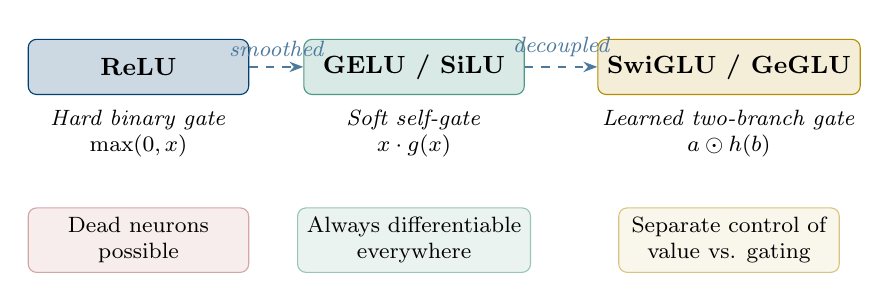
\begin{tikzpicture}[
  box/.style={rectangle, rounded corners=3pt, draw=keyblue!60, fill=keyblue!6, 
              minimum width=2.8cm, minimum height=0.7cm, align=center, font=\small},
  arrow/.style={-{Stealth[length=5pt]}, thick, keyblue!70},
  label/.style={font=\footnotesize\itshape, color=keyblue!70}
]
% Column headers
\node[box, fill=keyblue!20, draw=keyblue, font=\small\bfseries] (r1) at (0,0) {ReLU};
\node[box, fill=emerald!15, draw=emerald!70, font=\small\bfseries] (r2) at (3.5,0) {GELU / SiLU};
\node[box, fill=accentgold!15, draw=accentgold, font=\small\bfseries] (r3) at (7.5,0) {SwiGLU / GeGLU};

% Descriptions
\node[align=center, font=\footnotesize] at (0,-0.85)   {\textit{Hard binary gate}\\$\max(0,x)$};
\node[align=center, font=\footnotesize] at (3.5,-0.85) {\textit{Soft self-gate}\\$x \cdot g(x)$};
\node[align=center, font=\footnotesize] at (7.5,-0.85) {\textit{Learned two-branch gate}\\$a \odot h(b)$};

% Properties row
\node[box, fill=darkred!8, draw=darkred!40, font=\footnotesize] (p1) at (0,-2.2)   {Dead neurons\\possible};
\node[box, fill=emerald!8, draw=emerald!40, font=\footnotesize] (p2) at (3.5,-2.2) {Always differentiable\\everywhere};
\node[box, fill=accentgold!8, draw=accentgold!50, font=\footnotesize] (p3) at (7.5,-2.2) {Separate control of\\value vs. gating};

% Evolution arrows
\draw[arrow, dashed] (r1.east) -- node[above, label]{smoothed} (r2.west);
\draw[arrow, dashed] (r2.east) -- node[above, label]{decoupled} (r3.west);
\end{tikzpicture}
\end{center}

%% ════════════════════════════════════════════════════════════════════════════
\section{Why Negative Outputs and Centering Matter}
\label{sec:centering}
%% ════════════════════════════════════════════════════════════════════════════

\subsection{Non-Centered ReLU Outputs}

Since $\mathrm{ReLU}(x) \ge 0$, hidden activations in ReLU networks carry a positive mean. For one neuron, $g_i = \delta a_i$. If $a_i \ge 0$ for all $i$, all gradient coordinates share the sign of $\delta$.

\begin{proposition}
If $a_i \ge 0$ a.s.\ for all $i$, then for any sample with $\delta \ne 0$, all nonzero $g_i$ share the sign of $\delta$.
\end{proposition}
\begin{proof}
$g_i = \delta a_i$; since $a_i \ge 0$, $\mathrm{sgn}(g_i) = \mathrm{sgn}(\delta)$ whenever $a_i>0$.
\end{proof}

This means gradient updates are forced to lie in an orthant — a severe restriction on optimization direction diversity.

\begin{critbox}[Gap in Original: ELU Mean]
The original claims ELU outputs are ``centered around zero.'' This is only approximately true. The mean of ELU$(x)$ under typical initialization distributions is slightly negative (due to the $\alpha(e^x-1)$ tail), not exactly zero. Exact centering requires BatchNorm or explicit output normalization.
\end{critbox}

\subsection{Mean Decomposition}

For the activation vector $a$ with mean $\mu = \E[a]$:
\[
\E[a a^\top] = \Cov(a) + \mu\mu^\top.
\]
The rank-one term $\mu\mu^\top$ is the precise source of mean-induced gradient alignment.

\begin{keybox}
Centering matters not because negative values carry ``more information'' — it matters because $\mu = 0$ eliminates the $\mu\mu^\top$ term, reducing the dominant direction bias in gradient statistics.
\end{keybox}

%% ════════════════════════════════════════════════════════════════════════════
\section{Correlated Gradient Updates}
\label{sec:corr}
%% ════════════════════════════════════════════════════════════════════════════

\subsection{Exact Covariance}

\[
\Cov(g_i, g_j) = \E[\delta^2 a_i a_j] - \E[\delta a_i]\E[\delta a_j].
\]

\subsection{Approximate Decomposition}

Under weak dependence between $\delta$ and $(a_i, a_j)$:
\[
\Cov(g_i,g_j) \approx \underbrace{\E[\delta^2]\Cov(a_i,a_j)}_{\text{activation covariance}} + \underbrace{\Var(\delta)\E[a_i]\E[a_j]}_{\text{mean-induced term}}.
\]

\begin{critbox}[Gap: Approximation Validity]
The decomposition above assumes $\delta$ is approximately independent of $(a_i,a_j)$. In deep networks this fails in later layers where $\delta$ is a complex function of activations. The exact identity always holds; the decomposition is a pedagogical approximation. Practitioners should be aware the mean-induced term may be offset or amplified by $\delta$--$a$ coupling.
\end{critbox}

\begin{critbox}[Distinction: Magnitude vs.\ Direction]
Correlated gradient updates are \emph{distinct} from vanishing gradients. Vanishing gradients concern gradient \textbf{magnitude}; correlated updates concern gradient \textbf{directional diversity}. A network can have large but highly correlated gradients, wasting compute without improving optimization.
\end{critbox}

%% ════════════════════════════════════════════════════════════════════════════
\section{Optimization Geometry and Conditioning}
%% ════════════════════════════════════════════════════════════════════════════

\subsection{Quadratic Approximation}

Near $\theta$:
\[
L(\theta + \Delta) \approx L(\theta) + \nabla L(\theta)^\top \Delta + \tfrac{1}{2}\Delta^\top H(\theta)\Delta,
\]
where $H(\theta) = \nabla^2 L(\theta)$ is the Hessian.

\subsection{Condition Number}

\[
\kappa(H) = \frac{\lambda_{\max}(H)}{\lambda_{\min}(H)}.
\]

\begin{proposition}
For gradient descent on a strictly convex quadratic with step size $\eta^* = 2/(\lambda_{\max}+\lambda_{\min})$, convergence satisfies
\[
\norm{e_t} \le \left(\frac{\kappa-1}{\kappa+1}\right)^t \norm{e_0}.
\]
\end{proposition}

The ratio $(\kappa-1)/(\kappa+1) \to 1$ as $\kappa \to \infty$, confirming that poor conditioning causes convergence to stall.

\subsection{Mean Shift Amplifies Ill-Conditioning}

For $M = \Sigma + \mu\mu^\top$, $\lambda_{\max}(M) \ge \norm{\mu}^2$. Non-centered activations therefore directly inflate the spectral spread of curvature-related matrices, worsening the condition number.

\begin{keybox}
Non-centered activations worsen optimization not by removing gradients, but by increasing \textbf{anisotropy}: updates become directionally biased, and the effective condition number grows.
\end{keybox}

%% ════════════════════════════════════════════════════════════════════════════
\section{Batch Normalization}
%% ════════════════════════════════════════════════════════════════════════════

\subsection{Definition}

For feature coordinate $a_j$:
\[
\hat{a}_j = \frac{a_j - \mu_{B,j}}{\sqrt{\sigma_{B,j}^2 + \varepsilon}}, \qquad y_j = \gamma_j \hat{a}_j + \beta_j.
\]

\subsection{Effect}

Ignoring the learned affine transform: $\E_B[\hat{a}_j] \approx 0$, $\Var_B(\hat{a}_j) \approx 1$. This directly zeros out $\mu$ in the mean decomposition $\E[aa^\top] = \Cov(a) + \mu\mu^\top$, eliminating the rank-one bias term.

\begin{critbox}[Gap: BatchNorm vs.\ LayerNorm]
The original covers BatchNorm exclusively. In practice, \textbf{Layer Normalization} (normalizing across features for a single sample) is standard in transformers, where batch statistics are unreliable due to autoregressive masking and long-sequence batching. LayerNorm achieves similar centering and scaling benefits without batch-size dependence. \textbf{RMSNorm} (used in LLaMA) further simplifies by normalizing by RMS only, omitting the mean subtraction.
\end{critbox}

\begin{practbox}[Normalization Choices]
\begin{tabular}{@{}lll@{}}
\toprule
\textbf{Method} & \textbf{Normalization axis} & \textbf{Typical use} \\
\midrule
BatchNorm  & Batch dimension per feature  & CNNs, image models \\
LayerNorm  & Feature dimension per sample & Transformers \\
RMSNorm    & Feature dimension (RMS only) & LLaMA, modern LLMs \\
GroupNorm  & Feature groups per sample    & Detection, small batch \\
\bottomrule
\end{tabular}
\end{practbox}

%% ════════════════════════════════════════════════════════════════════════════
\section{Second-Order Structure and Gauss--Newton}
%% ════════════════════════════════════════════════════════════════════════════

\subsection{Gauss--Newton Matrix}

For $L(\theta) = \frac{1}{2}\norm{r(\theta)}^2$ with Jacobian $J \in \R^{M \times p}$:
\[
G(\theta) = J^\top J \succeq 0.
\]

\subsection{Kronecker Structure of Gradient Second Moments}

Using $\mathrm{vec}(\nabla_W L) = a \otimes \delta$:
\[
\E\!\left[\mathrm{vec}(\nabla_W L)\,\mathrm{vec}(\nabla_W L)^\top\right]
= \E\!\left[(aa^\top) \otimes (\delta\delta^\top)\right]
\approx \E[aa^\top] \otimes \E[\delta\delta^\top].
\]

\begin{proposition}
For $A,B \succ 0$: $\kappa(A \otimes B) = \kappa(A)\,\kappa(B).$
\end{proposition}
\begin{proof}
Eigenvalues of $A \otimes B$ are all products $\lambda_i(A)\lambda_j(B)$, so
\[
\kappa(A\otimes B) = \frac{\lambda_{\max}(A)\lambda_{\max}(B)}{\lambda_{\min}(A)\lambda_{\min}(B)} = \kappa(A)\kappa(B).
\]
\end{proof}

\begin{keybox}[Conditioning Multiplies Across Factors]
Anisotropy in activations and anisotropy in error signals \emph{multiply} in parameter space. This motivates K-FAC (Kronecker-factored approximate curvature) as a practical second-order optimizer.
\end{keybox}

%% ════════════════════════════════════════════════════════════════════════════
\section{Adaptive Optimization: Adam and AdamW}
%% ════════════════════════════════════════════════════════════════════════════

\subsection{Adam}

Adam maintains exponential moving averages of gradients ($m_t$) and squared gradients ($v_t$):
\[
m_t = \beta_1 m_{t-1} + (1-\beta_1)g_t, \qquad
v_t = \beta_2 v_{t-1} + (1-\beta_2)g_t^{\odot 2},
\]
with bias corrections $\hat{m}_t = m_t/(1-\beta_1^t)$, $\hat{v}_t = v_t/(1-\beta_2^t)$, and update:
\[
\theta_{t+1} = \theta_t - \eta\,\frac{\hat{m}_t}{\sqrt{\hat{v}_t}+\varepsilon}.
\]

\subsection{AdamW: Decoupled Weight Decay}

\begin{critbox}[Gap in Original: Adam vs.\ AdamW]
The original covers Adam but omits \textbf{AdamW}, which is now the standard in LLM training. Standard Adam applies weight decay as $L_2$ regularization added to the gradient, which is scaled by $1/\sqrt{\hat{v}_t}$ — making weight decay smaller for parameters with large historical gradients. AdamW decouples weight decay from the gradient update:
\[
\theta_{t+1} = (1 - \eta\lambda)\,\theta_t - \eta\,\frac{\hat{m}_t}{\sqrt{\hat{v}_t}+\varepsilon},
\]
so weight decay acts uniformly regardless of gradient history. This distinction matters practically: AdamW generalizes substantially better in transformer training.
\end{critbox}

\begin{practbox}[Adam Hyperparameter Guidance]
Typical defaults: $\beta_1 = 0.9$, $\beta_2 = 0.999$, $\varepsilon = 10^{-8}$. For LLM training: $\beta_2 = 0.95$ is often preferred to track gradient variance faster. $\varepsilon = 10^{-6}$ or larger can improve stability in mixed-precision training.
\end{practbox}

\subsection{Limitations of Diagonal Preconditioning}

\begin{keybox}
Adam normalizes each coordinate independently, approximating diagonal inverse curvature. It cannot correct \textbf{off-diagonal coupling} in the true Hessian. K-FAC and Shampoo address off-diagonal structure but are more expensive to compute.
\end{keybox}

%% ════════════════════════════════════════════════════════════════════════════
\section{Residual Connections and Gradient Transport}
%% ════════════════════════════════════════════════════════════════════════════

\subsection{Plain Network: Vanishing Product}

In a plain network $x_{\ell+1} = F_\ell(x_\ell)$:
\[
\frac{\partial x_L}{\partial x_0} = \prod_{\ell=0}^{L-1} J_\ell, \qquad J_\ell = \frac{\partial F_\ell}{\partial x_\ell}.
\]
If $\|J_\ell\| < 1$ for all $\ell$, this product vanishes exponentially.

\subsection{Residual Block}

For $x_{\ell+1} = x_\ell + F_\ell(x_\ell)$:
\[
\frac{\partial x_{\ell+1}}{\partial x_\ell} = I + J_\ell.
\]

\begin{proposition}
If each $\|J_\ell\|$ is small, $I + J_\ell$ remains close to identity, stabilizing gradient transport.
\end{proposition}

The product $\prod_\ell(I + J_\ell)$ expands into a sum over all subsets of residual corrections — the gradient sees a direct path (the identity) plus higher-order terms, preventing exponential vanishing.

\begin{critbox}[Gap: Gradient Explosion Risk]
The original focuses on vanishing but not explosion. Residual connections also risk \textbf{gradient explosion} when $\|J_\ell\| \gg 0$ since $\|I + J_\ell\| \le 1 + \|J_\ell\|$. Gradient clipping (clipping gradient norm to a threshold, e.g., 1.0) is standard practice in deep residual and transformer training precisely to prevent this.
\end{critbox}

\begin{keybox}
Residual connections replace a pure product of Jacobians with a product of \textbf{perturbations of the identity}, providing gradient superhighways through depth. Gradient clipping guards against the explosion side of this trade-off.
\end{keybox}

\begin{center}
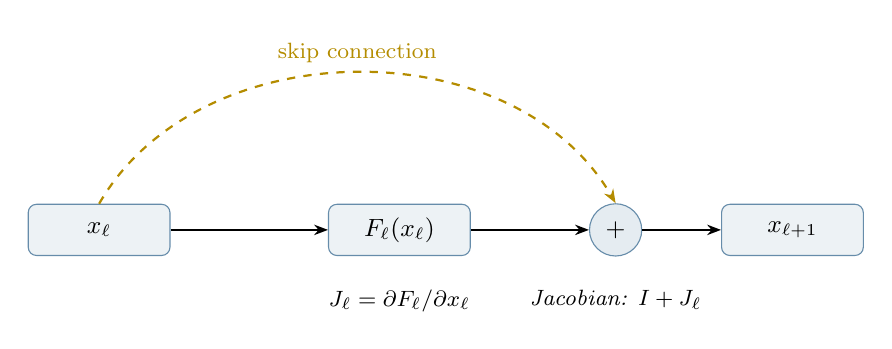
\begin{tikzpicture}[
  node distance=1.4cm,
  block/.style={rectangle, rounded corners=3pt, draw=keyblue!60, fill=keyblue!7,
                minimum width=1.8cm, minimum height=0.65cm, font=\small, align=center},
  arrow/.style={-{Stealth[length=5pt]}, thick},
  skip/.style={-{Stealth[length=5pt]}, thick, accentgold, dashed}
]
\node[block] (x0) {$x_\ell$};
\node[block, right=2cm of x0] (f) {$F_\ell(x_\ell)$};
\node[circle, draw=keyblue!60, fill=keyblue!10, right=1.5cm of f, minimum size=0.55cm, font=\small] (plus) {$+$};
\node[block, right=1cm of plus] (x1) {$x_{\ell+1}$};

\draw[arrow] (x0) -- (f);
\draw[arrow] (f) -- (plus);
\draw[arrow] (plus) -- (x1);
\draw[skip] (x0.north) to[out=60,in=120] node[above,font=\footnotesize\color{accentgold}]{skip connection} (plus.north);

\node[font=\footnotesize\itshape, below=0.3cm of f] {$J_\ell = \partial F_\ell/\partial x_\ell$};
\node[font=\footnotesize\itshape, below=0.3cm of plus] {Jacobian: $I + J_\ell$};
\end{tikzpicture}
\end{center}

%% ════════════════════════════════════════════════════════════════════════════
\section{Neural Tangent Kernel Regime}
%% ════════════════════════════════════════════════════════════════════════════

\subsection{Definition}

\[
\Theta_\theta(x, x') = \nabla_\theta f_\theta(x)^\top \nabla_\theta f_\theta(x').
\]

\subsection{Infinite-Width Limit}

In the infinite-width limit, $\Theta_\theta$ converges at initialization to a deterministic kernel $\Theta^*$ and remains approximately constant during training. Gradient descent then evolves the outputs as:
\[
\frac{d}{dt}f_\theta(x) = -\Theta^*(x,\cdot)\bigl(f_\theta(\cdot) - y\bigr),
\]
a linear kernel regression in function space.

\begin{critbox}[Gap: NTK Regime vs.\ Feature Learning]
The NTK regime is \textbf{not} how modern large models behave. It describes an extreme of near-infinite width; practical networks operate in a ``feature learning'' (or ``rich'') regime where kernels change substantially during training. The NTK is a theoretical tool — it proves convergence for overparameterized networks and connects to kernel methods, but practitioners should not expect their models to be in the NTK regime.
\end{critbox}

%% ════════════════════════════════════════════════════════════════════════════
\section{Implicit Bias of Gradient Descent}
%% ════════════════════════════════════════════════════════════════════════════

\subsection{The Phenomenon}

Optimization algorithms prefer certain solutions even without explicit regularization. For underdetermined linear regression with GD initialized at zero, the solution converges to the minimum Euclidean norm interpolant:
\[
\theta^* = \arg\min_\theta \norm{\theta}_2 \quad \text{s.t.} \quad X\theta = y.
\]

\subsection{Extensions}

\begin{practbox}[Implicit Bias in Modern Settings]
\begin{itemize}
    \item \textbf{Matrix factorization}: GD on $UV^\top$ biases toward low-rank solutions.
    \item \textbf{Diagonal networks}: GD biases toward sparse solutions.
    \item \textbf{Transformers}: Evidence of inductive biases toward attention to simple token patterns at early layers; the exact characterization is an open research area.
    \item \textbf{Label smoothing and dropout} interact with implicit bias by perturbing the loss landscape.
\end{itemize}
\end{practbox}

\begin{keybox}
Implicit bias connects optimization to generalization. Architectural and optimizer choices shape \emph{which} solution is found, not merely \emph{whether} training converges.
\end{keybox}

%% ════════════════════════════════════════════════════════════════════════════
\section{Unified Synthesis}
%% ════════════════════════════════════════════════════════════════════════════

\begin{mytheorem}{Unified Optimization Principle}{unified}
Efficient gradient-based training of deep neural networks is promoted by:
\begin{enumerate}
    \item activation derivatives not systematically small (ReLU $\to$ GELU/SiLU),
    \item hidden activations centered and well-scaled through normalization (BatchNorm/LayerNorm),
    \item sufficient curvature conditioning (AdamW preconditioning),
    \item stable depthwise gradient transport (residual connections + gradient clipping),
    \item coordinatewise gradient scales moderated by adaptive preconditioning,
    \item expressive feature-gating mechanisms where needed (SwiGLU/GeGLU in FFN blocks).
\end{enumerate}
Training deteriorates when any of these conditions are violated.
\end{mytheorem}

\vspace{10pt}
\begin{center}
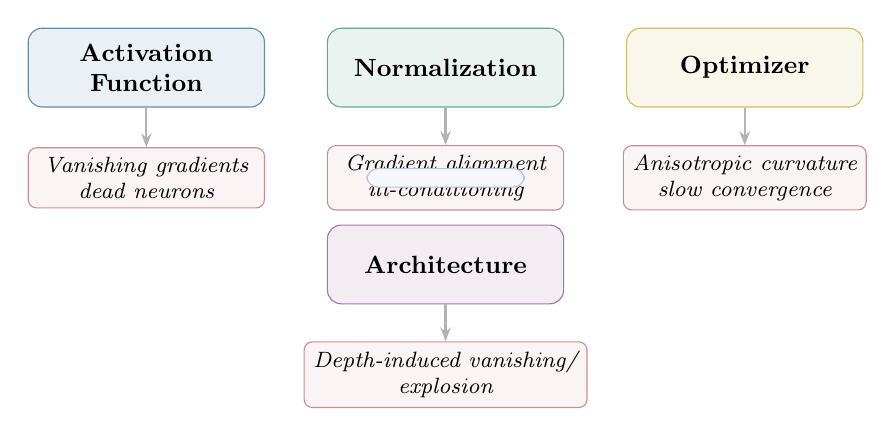
\begin{tikzpicture}[
  comp/.style={rectangle, rounded corners=5pt, draw=#1!60, fill=#1!8,
               minimum width=3.0cm, minimum height=1.0cm, align=center, font=\small\bfseries},
  prob/.style={rectangle, rounded corners=3pt, draw=darkred!50, fill=darkred!5,
               minimum width=3.0cm, minimum height=0.65cm, align=center, font=\footnotesize\itshape},
  arrow/.style={-{Stealth[length=5pt]}, thick, gray!60},
  connects/.style={thick, gray!40, dashed}
]
% Row 1: Components
\node[comp=keyblue]   (act) at (0,0)     {Activation\\Function};
\node[comp=emerald]   (norm) at (3.8,0)  {Normalization};
\node[comp=accentgold](opt) at (7.6,0)   {Optimizer};
\node[comp=plum]      (arch) at (3.8,-2.5){Architecture};

% Row 2: What they fix
\node[prob] (p1) at (0,-1.4)    {Vanishing gradients\\dead neurons};
\node[prob] (p2) at (3.8,-1.4)  {Gradient alignment\\ill-conditioning};
\node[prob] (p3) at (7.6,-1.4)  {Anisotropic curvature\\slow convergence};
\node[prob] (p4) at (3.8,-3.9)  {Depth-induced vanishing/\\explosion};

\draw[arrow] (act.south) -- (p1.north);
\draw[arrow] (norm.south) -- (p2.north);
\draw[arrow] (opt.south) -- (p3.north);
\draw[arrow] (arch.south) -- (p4.north);

% Central label
\node[rectangle, draw=keyblue!30, fill=keyblue!4, rounded corners=4pt,
      font=\small\bfseries\color{keyblue}, minimum width=2.0cm] at (3.8,-1.4+0.0) {};
\end{tikzpicture}
\end{center}

%% ════════════════════════════════════════════════════════════════════════════
\section{Conclusion}
%% ════════════════════════════════════════════════════════════════════════════

The optimization of deep neural networks cannot be understood through any single concept. The following table summarizes the full picture:

\vspace{6pt}
\renewcommand{\arraystretch}{1.18}
\begin{center}
\begin{tabularx}{0.96\textwidth}{@{}>{\raggedright\arraybackslash}p{3.2cm}>{\raggedright\arraybackslash}X>{\raggedright\arraybackslash}p{3.9cm}@{}}
\toprule
\textbf{Component} & \textbf{Role} & \textbf{Failure mode addressed} \\
\midrule
Sigmoid     & Historical baseline & Vanishing gradients, mean shift \\
ReLU        & Gradient preservation in active region & Magnitude vanishing \\
Leaky ReLU / ELU & Nonzero negative-side derivative & Dead neurons \\
GELU        & Smooth probabilistic gate ($x\Phi(x)$) & Kink, dead neurons, smoothness \\
SiLU/Swish  & Smooth sigmoid self-gate ($x\sigma(x)$) & Kink, dead neurons \\
SwiGLU / GeGLU & Two-branch learned gate & Feature expressivity, gradient coupling \\
\midrule
BatchNorm   & Zero mean, unit variance per batch & Gradient alignment, scale \\
LayerNorm   & Zero mean per sample & Same, sequence-model safe \\
RMSNorm     & Scale only, no mean subtraction & Simplified LayerNorm \\
\midrule
Adam        & Diagonal adaptive preconditioning & Anisotropic curvature \\
AdamW       & Decoupled weight decay & Generalization \\
\midrule
Residual connections & $I + J_\ell$ Jacobian & Gradient vanishing with depth \\
Gradient clipping & Norm bound on updates & Gradient explosion \\
\midrule
NTK theory  & Kernel view of wide networks & Convergence guarantees \\
Implicit bias & Solution selection geometry & Generalization \\
\bottomrule
\end{tabularx}
\end{center}

\vspace{10pt}
\begin{keybox}[Final Takeaway]
Deep learning works well in practice because modern architectures and optimizers \textbf{jointly} control gradient magnitude, gradient direction, curvature, and transport across depth. Each design choice — GELU over ReLU, SwiGLU in FFN blocks, LayerNorm, AdamW, skip connections — addresses a specific, mathematically identifiable failure mode. Understanding the mathematics makes these choices transparent rather than empirical folklore.
\end{keybox}

\end{document}
